\documentclass[12pt]{article}
\usepackage[english]{babel}
\usepackage[utf8]{inputenc}
\usepackage{amsmath, amssymb, amsthm}
\usepackage{graphicx}
\usepackage{hyperref}
\usepackage[margin=.75in]{geometry}
\usepackage{xcolor}
\usepackage{tikz}

\newcommand{\id}{\text{id}}
\newcommand{\od}{\text{od}}

\setlength{\topmargin}{0pt}
\setlength{\headsep}{0pt}
\textheight = 600pt

\title{Graph Theory \\ Homework 16}
\author{Ben Kallus and Josef Komissar}
\date{Due Monday, April 26}

\begin{document}
\maketitle

\medskip\noindent\textbf{I (a)}

    We have previously shown that $Q_n$ is bipartite for all $n \in \mathbb N$.
    Thus, by K\"onig's Theorem, $\chi'(Q_n) = \Delta(Q_n) = n$.

\medskip\noindent\textbf{I (b)}

    The maximum vertex degree in the Gr\"otzsch graph is 5, so by Vizing's Theorem, the chromatic index of the Gr\"otzsch graph is either 5 or 6.
    The following drawing shows that the chromatic index of the Gr\"otzsch graph is 5.
    \begin{center} 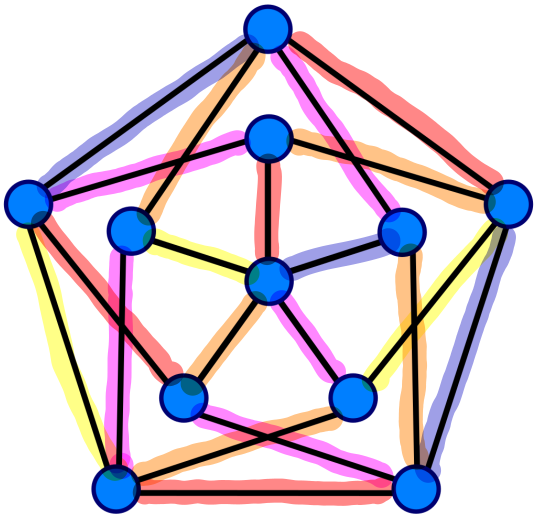
\includegraphics[scale=.5]{fig1.png} \end{center}

\medskip\noindent\textbf{I (c)}

    By Theorem 8.13, PG is not 1-factorable.
    Because PG is regular, by the special case we discussed in class following Theorem 10.13, $\chi'(PG) \neq 3$, so $\chi'(PG) = 4$.

\medskip\noindent\textbf{10.18} Proposition: If $H$ is a $2k$-regular graph of order $4k+1$ for some positive integer $k$, and $G$ is a subgraph of $H$ obtained by removing a set of $k-1$ independent edges from $H$, then $\chi'(G) = \Delta(G) + 1$.
\begin{proof}
    Let $k \in \mathbb Z^+$, and let $H$ be a $2k$-regular graph of order $n = 4k+1$.
    Let $G$ be a subgraph of $H$ obtained by removing a set of $k-1$ independent edges from $H$.
    Then, by the Handshaking Lemma, $|E(G)| = \frac{2k(4k+1)}{2} - (k-1) = 4k^2 + 1$.
    Thus,
    \begin{align*}
        |E(G)| &= 4k^2 + 1 \\
        &> 4k^2 \\
        &= \frac12 \cdot 2k \cdot 4k \\
        &= \frac12 \Delta(H) (n - 1) \\
        &\geq \frac12\Delta(G)(n-1).
    \end{align*}

    Thus, by Theorem 10.13, $\chi'(G) = 1 + \Delta(G)$.
\end{proof}

\medskip\noindent\textbf{II (a)} Proposition: If $G$ is a graph in which every vertex except one has degree $d \geq 1$, and $\chi'(G) = d$, then $G$ has odd order.
\begin{proof}
    Let $G$ be a graph in which every vertex except one has degree $d \geq 1$.
    Let $u$ be the vertex in $G$ that does not have degree $d$.
    Suppose that $\chi'(G) = d$.
    Suppose that $\deg(u) > d$.
    Then, each edge incident to $u$ must have a distinct color.
    Thus, $\chi'(G) > d$, which contradicts our assumption.
    Thus, $\deg(u) < d$.
    Because $\deg(u) < \chi'(G)$, there exists a color $c$ in a $d$-coloring of $G$ such that no $c$-colored edge is incident to $u$.
    Consider the set of all $c$-colored edges in $G$.
    Because all vertices in $G - u$ have degree $d$, and $\chi'(G) = d$, each of these vertices must be incident to exactly one $c$-colored edge.
    Thus, because the $c$-colored edges are independent, they constitute a perfect matching on $G-u$.
    Thus, $G-u$ has even order, so $G$ has odd order.
\end{proof}

\medskip\noindent\textbf{II (b)} Proposition: If $G$ is a graph in which every vertex except one has degree $d \geq 1$, and $\chi'(G) = d$, then $G$ has an isolated vertex.
\begin{proof}
    Let $G$ be a graph in which every vertex except one has degree $d \geq 1$.
    Let $u$ be the vertex in $G$ that does not have degree $d$.
    Suppose that $\chi'(G) = d$.
    Suppose that $\deg(u) > 0$.
    Then, there exists a color $c$ in a $d$-coloring of $G$ such that an edge of color $c$ is incident to $u$.
    Note that because $\chi'(G) = d$, and $\deg(v) = d$ for all $v \in V(G) \setminus \{u\}$, there exists a $c$-colored edge incident to each of these vertices.
    Thus, the set of all $c$-colored edges in $G$ induces a perfect matching in $G$.
    However, $G$ is of odd order, so it cannot have a perfect matching.
    Thus, $\deg(u) = 0$.
\end{proof}

\medskip\noindent\textbf{III} Proposition: If $G$ is a connected $d$-regular graph and $u$ is a cut-vertex of $G$, then $\chi'(G) = d+1$.
\begin{proof}
    Let $d \geq 1$, and let $G$ be a connected $d$-regular graph with cut-vertex $u$.
    Let $H$ be a component of $G-u$.
    Then, every edge that runs between a vertex in $H$ and a vertex in $G-H$ must be incident to $u$.
    Note that because $u$ is a cut-vertex, $u$ must be adjacent to at least one vertex $v$ in $G-H$.
    Thus, $G-H$ is connected, because the only vertex in $G-H$ that was affected by $H$'s removal is $u$, and $u$ is adjacent to $v$ in $G-H$.
    Then, every vertex in $G-H$ has degree $d$ except $u$.

    Suppose that $\chi'(G-H) = d$.
    Then, by \textbf{II (b)}, $G - H$ has an isolated vertex.
    This contradicts its connectedness, so $\chi'(G-H) = d+1$.
    Thus, $\chi'(G) \geq d+1$.
    Thus, by Vizing's Theorem, $\chi'(G) = d + 1$.
\end{proof}

\medskip\noindent\textbf{IV}
\begin{proof}
    9.15 says $\delta(G) \leq 4$ and $\delta(G') \leq 4$ for all $g' \subseteq G$. (because $g'$ would also be planar and of order $\leq 11$.
    Then, by 10.9, $\chi(G) \leq 5$.
\end{proof}

\medskip\noindent\textbf{V}


\end{document}
